\chapter{Degradation Case Study and Recovery Results}
\label{chap:degradation-case-study}

\section{Transient versus sustained degradation}
\label{sec:transient-provider-degradation}

A drop in accuracy on $\mathcal{D}_n$ does not necessarily indicate lasting degradation. For example, on 22–23 March 2026, \texttt{gpt-4.1-mini} briefly underperformed \texttt{gpt-4.1-nano} but recovered within two days without intervention. As it was not deployed, no action was taken.

This motivates distinguishing transient from sustained degradation. Transient drops may resolve on their own, while sustained ones require intervention (Chapter~\ref{chap:prompt-optimisation}). In the monitoring protocol, the recommended response to an initial alert is therefore to switch to a fallback model and continue observing; prompt optimisation is triggered only if the regression persists across multiple evaluation windows.

Figure~\ref{fig:gpt41mini-transient-pit} shows the dashboard output on $\mathcal{D}_n$ for
8--28~March~2026. \texttt{gpt-4.1-mini} temporarily falls below \texttt{gpt-4.1-nano} on 22--23~March before recovering.

% Image is not versioned in this repository; place the export next to the thesis root if missing.

\begin{figure}[ht]
    \centering
    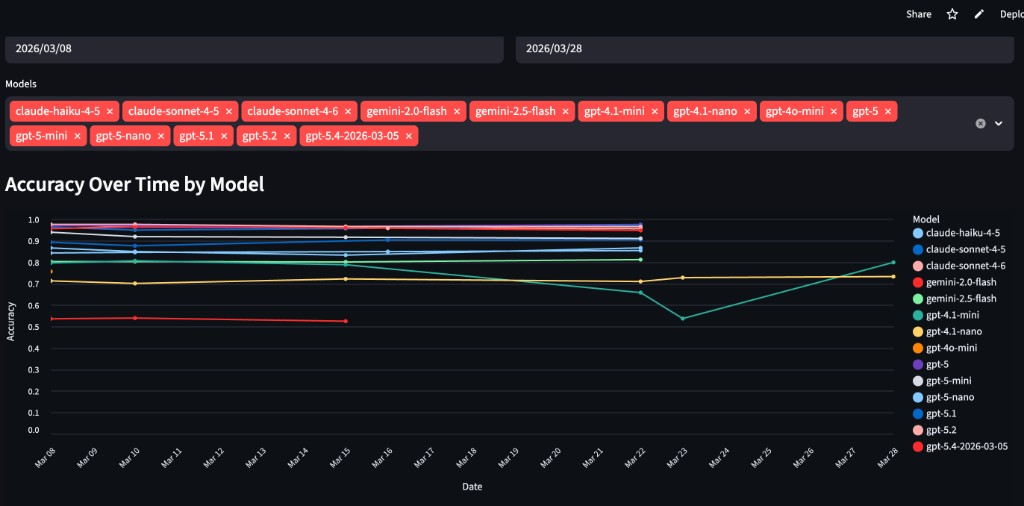
\includegraphics[width=\linewidth]{assets/gpt41mini-accuracy-pit-2026-03.png}
    \caption{Subset accuracy over time (monitoring dashboard). \texttt{gpt-4.1-mini} shows a temporary dip below \texttt{gpt-4.1-nano}, followed by recovery.}
    \label{fig:gpt41mini-transient-pit}
\end{figure}%


\section{Verified alert episode}
\label{sec:alerted-degradation-case}

\section{McNemar evidence at the trigger}
\label{sec:mcnemar-at-trigger}

\section{Metric and cost shift for the alternative model}
\label{sec:metric-alternative-comparison}

\section{Prompt optimisation results}
\label{sec:prompt-optimisation-results}

Figure~\ref{fig:gepa-opt-curve} shows the GEPA optimisation trajectory
obtained on \texttt{gpt-4.1-nano} for the campaign-relevance task. The
blue trace gives the aggregate validation score of each accepted
candidate on $D_{\mathrm{pareto}}$, and the orange trace reports the
running best. The seed prompt scores $0.65$; the best candidate
(iteration~4) reaches $0.867$, after which later accepted offspring
regress on the aggregate. This is consistent with the Pareto-based
selection rule of Section~\ref{sec:formal-gepa}: offspring that lose on
the average can still be retained if they dominate the incumbent on
specific instances, so the accepted-candidate curve is not monotone
even though the running best is.

\begin{figure}[ht]
    \centering
    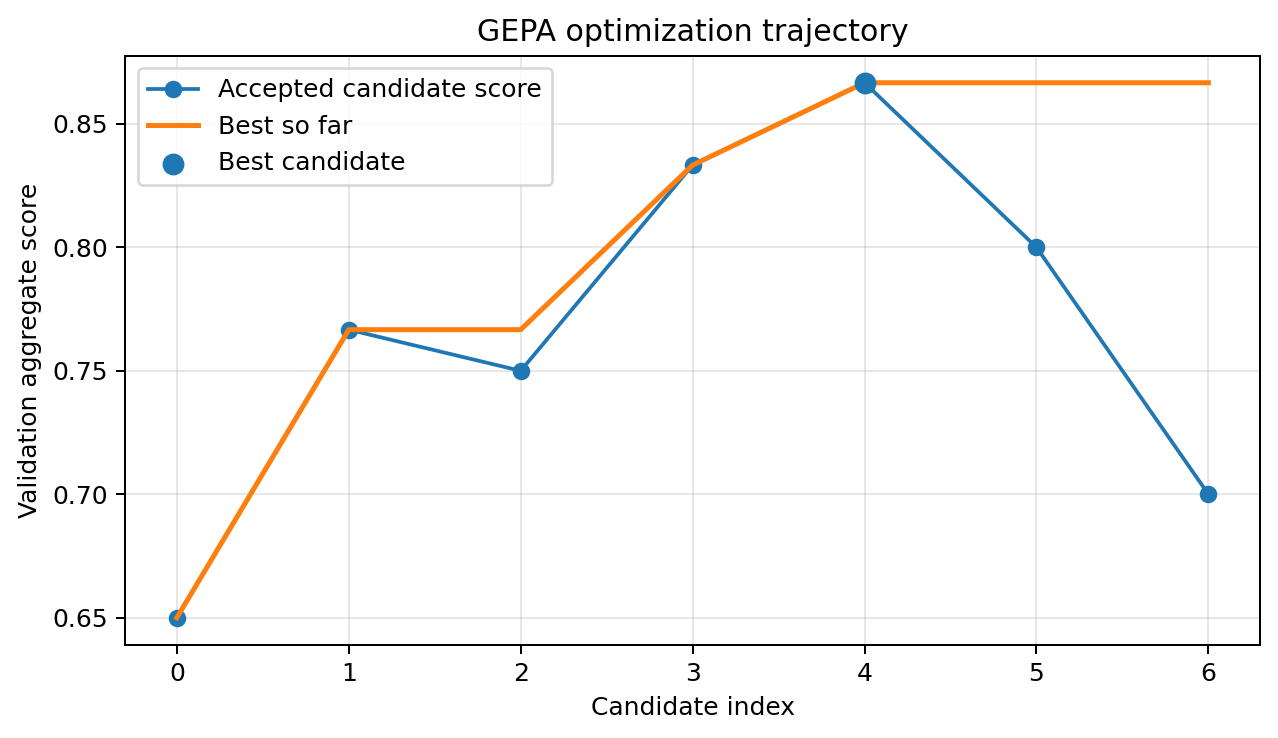
\includegraphics[width=0.85\linewidth]{assets/gepa_optimization_curve.png}
    \caption{GEPA optimisation trajectory on \texttt{gpt-4.1-nano}
    (campaign-relevance task). Blue: aggregate validation score of each
    accepted candidate on $D_{\mathrm{pareto}}$; orange: running best;
    filled marker: best candidate (iteration~4, score~$0.867$, up from
    $0.650$ at the seed prompt).}
    \label{fig:gepa-opt-curve}
\end{figure}
